\documentclass[11pt]{article}
\usepackage{amsmath}
\usepackage{booktabs}
\usepackage{tikz}

\title{How Many Times Can You Fold a Sheet of Paper?}
\author{An example project from TeXCraft}
\date{}

\begin{document}
\maketitle

\begin{abstract}
  Fold a sheet of paper in half, then in half again: each fold doubles its thickness, and
  after a few folds the paper refuses to bend. This short paper is TeXCraft's example
  project. It has sections in two files, a list, a table, a figure drawn with TikZ, numbered
  equations, cross-references and a citation, so you can see how each one is written. Change
  anything you like: the PDF follows as you type.
\end{abstract}

\section{Introduction}
It is often said that no sheet of paper can be folded in half more than seven or eight
times. The reason is simple to state:
\begin{itemize}
  \item each fold doubles the thickness (Section~\ref{sec:doubling});
  \item each fold also needs more paper to wrap around the ones before it;
  \item after a few folds, the stack is too short and too stiff to bend again.
\end{itemize}
This section is a file of its own, \texttt{sections/introduction.tex}, read with
\verb|\input|. Open it from the Files panel.


\section{Doubling}
\label{sec:doubling}
A sheet of thickness $t$ folded in half $n$ times is a stack of $2^n$ layers, so its
thickness is
\begin{equation}
  T_n = 2^n \, t .
  \label{eq:thickness}
\end{equation}
Office paper is about $0.1$~mm thick. Table~\ref{tab:folds} and Figure~\ref{fig:growth} show
how quickly \eqref{eq:thickness} grows.

\begin{table}[ht]
  \centering
  \begin{tabular}{rrl}
    \toprule
    Folds $n$ & Layers $2^n$ & Thickness $T_n$ \\
    \midrule
     1 &    2 & 0.2 mm \\
     4 &   16 & 1.6 mm \\
     7 &  128 & 12.8 mm, about a notebook \\
    10 & 1024 & 10.2 cm, a brick's width \\
    \bottomrule
  \end{tabular}
  \caption{The thickness of a folded sheet of office paper, from \eqref{eq:thickness}.}
  \label{tab:folds}
\end{table}

\begin{figure}[ht]
  \centering
  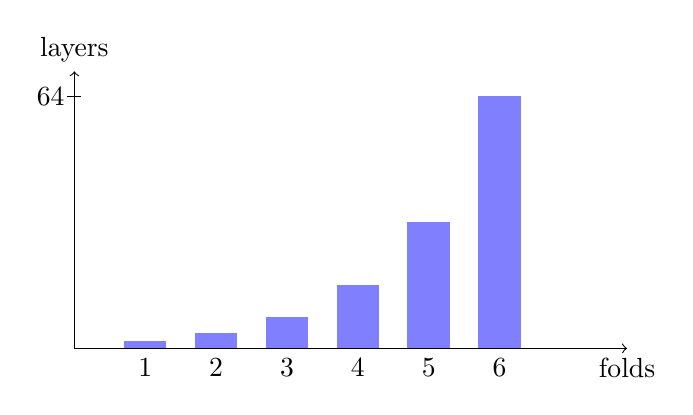
\begin{tikzpicture}[x=0.9cm, y=0.4cm]
    \draw[->] (0, 0) -- (7.8, 0) node[below] {folds};
    \draw[->] (0, 0) -- (0, 8.8) node[above] {layers};
    \foreach \n/\h in {1/0.25, 2/0.5, 3/1, 4/2, 5/4, 6/8} {
      \fill[blue!50] (\n - 0.3, 0) rectangle (\n + 0.3, \h);
      \node[below] at (\n, 0) {\n};
    }
    \node[left] at (0, 8) {64};
    \draw (-0.1, 8) -- (0.1, 8);
  \end{tikzpicture}
  \caption{Each fold doubles the number of layers.}
  \label{fig:growth}
\end{figure}

\section{Why the Folding Stops}
Folding also uses up length: the paper wraps around the fold, and the layers on the outside
travel further than those inside. For a long strip folded in one direction, the length
needed for $n$ folds is~\cite{gallivan2002}
\begin{equation}
  L_n = \frac{\pi t}{6} \left(2^n + 4\right)\left(2^n - 1\right).
  \label{eq:length}
\end{equation}
By \eqref{eq:length}, twelve folds of paper $0.1$~mm thick take a strip about 880 metres
long, while seven folds need less than one.

\bibliographystyle{plain}
\bibliography{references}

\end{document}
